\section{Figures} \label{sec:Figures}

\subsection*{A.1\quad Process Dynamics Illustration}

\begin{figure}[H]
    \centering
    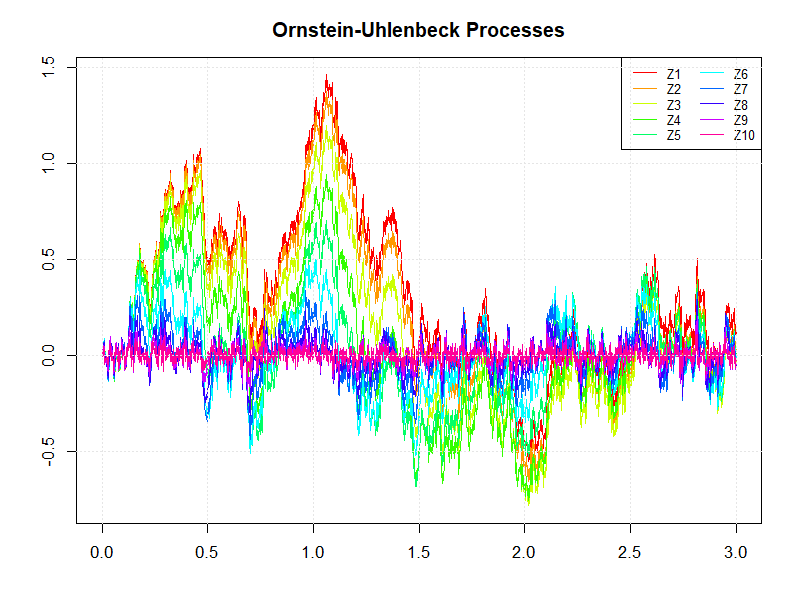
\includegraphics[width=0.75\textwidth]{figures/A.1 Process Dynamics/ou_processes.png}
    \caption{Sample Ornstein-Uhlenbeck processes with different mean-reversion speeds.}
    \label{fig:OUProcesses}
\end{figure}

\begin{figure}[H]
    \centering
    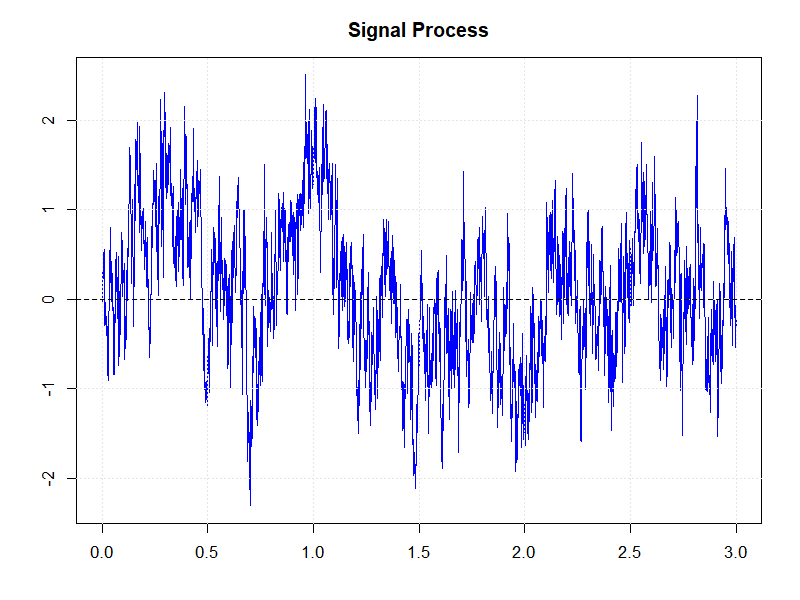
\includegraphics[width=0.75\textwidth]{figures/A.1 Process Dynamics/signal_process.png}
    \caption{Signal process obtained as a weighted combination of OU processes. The aggregation produces rough and persistent sample paths, consistent with empirical volatility dynamics.}
    \label{fig:SignalProcess}
\end{figure}

\begin{figure}[H]
    \centering
    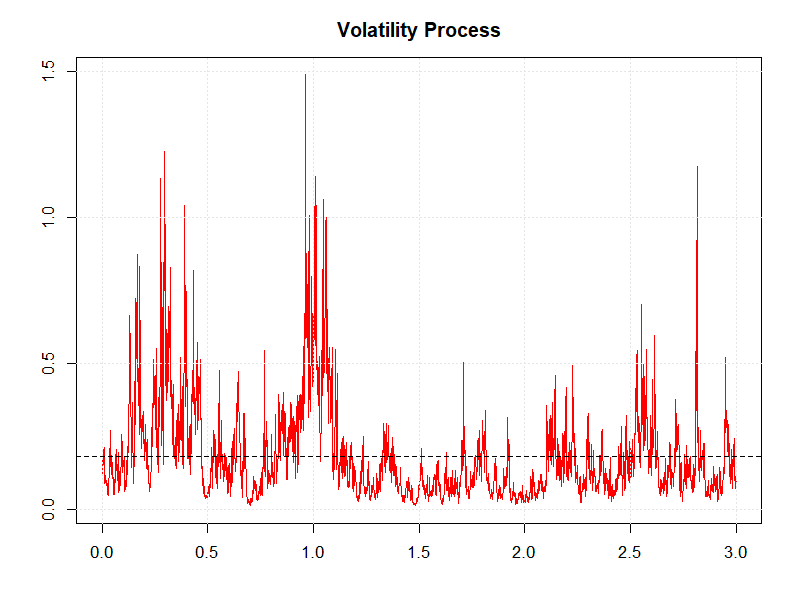
\includegraphics[width=0.75\textwidth]{figures/A.1 Process Dynamics/volatility_process.png}
    \caption{Volatility process derived via exponential transformation of the signal. The process remains strictly positive and exhibits clustering and occasional spikes.}
    \label{fig:VolatilityProcess}
\end{figure}

\begin{figure}[H]
    \centering
    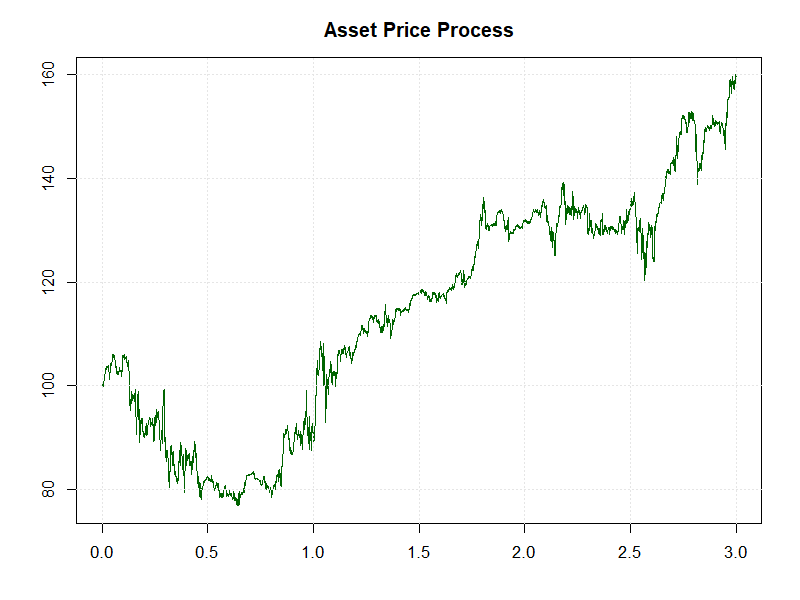
\includegraphics[width=0.75\textwidth]{figures/A.1 Process Dynamics/asset_price.png}
    \caption{Simulated asset price process driven by the stochastic volatility. The trajectory reflects both drift and volatility clustering effects.}
    \label{fig:AssetPrice}
\end{figure}



\newpage
\subsection*{A.2\quad Additional Market Surface}

To illustrate the stability of the empirical implied volatility surface across different sample periods, 
Figure~\ref{fig:MarketSurfaceApr2023} shows the S\&P~500 surface constructed from April 2023 option data. 
The same cleaning and interpolation procedures as described in Section~\ref{subsec:EmpiricalVolatilitySurface} 
were applied. The surface exhibits the same qualitative features as the March 2023 surface: convex volatility smiles, 
a negative and increasing ATM skew, and an approximate power-law decay in the skew term structure. 
This confirms that the stylized facts underlying the simulation quality criteria are consistently present 
in market data across different months.

\begin{figure}[H]
    \centering
    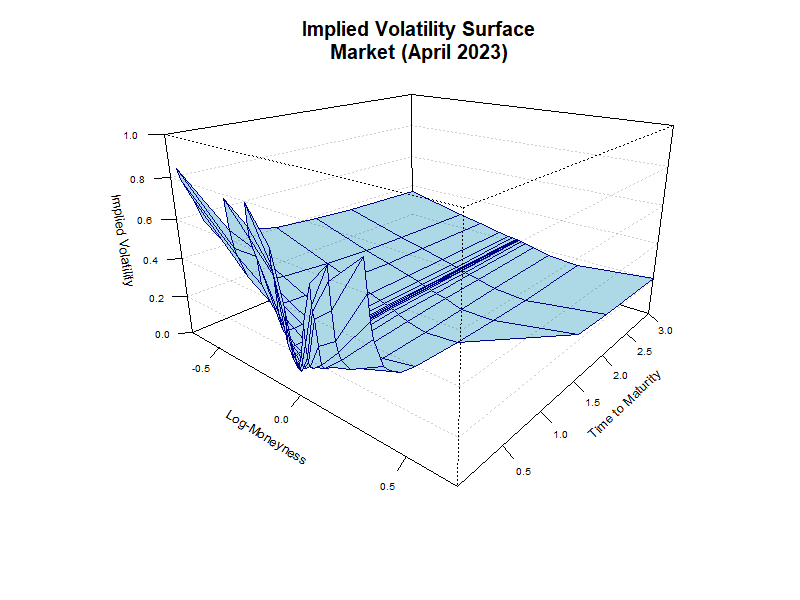
\includegraphics[width=0.45\textwidth]{figures/A.2 Additional Market Surface/market_apr-23_iv_surface.png}
    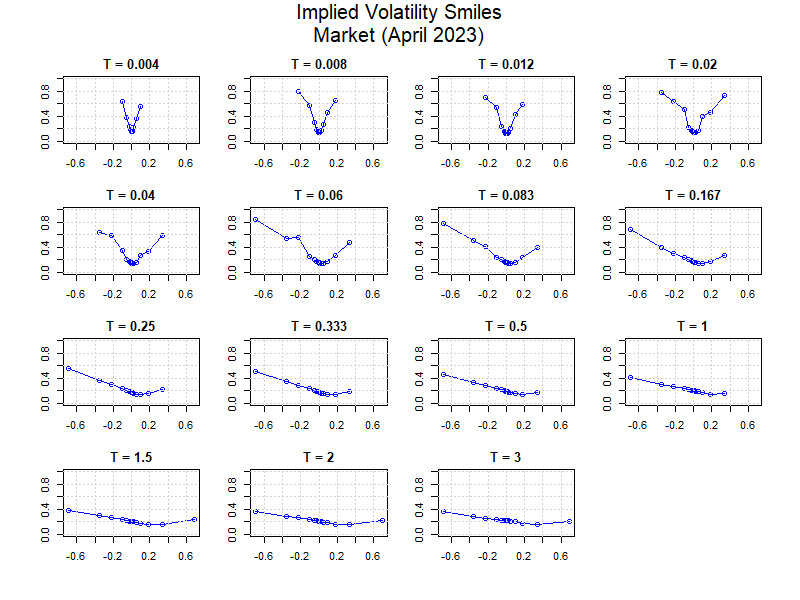
\includegraphics[width=0.45\textwidth]{figures/A.2 Additional Market Surface/market_apr-23_iv_smiles.png}
    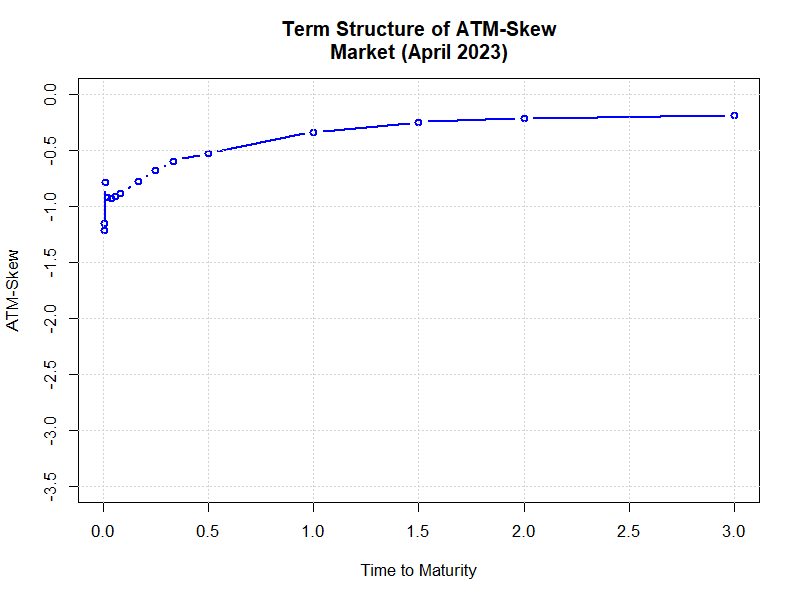
\includegraphics[width=0.45\textwidth]{figures/A.2 Additional Market Surface/market_apr-23_atm_skew.png}
    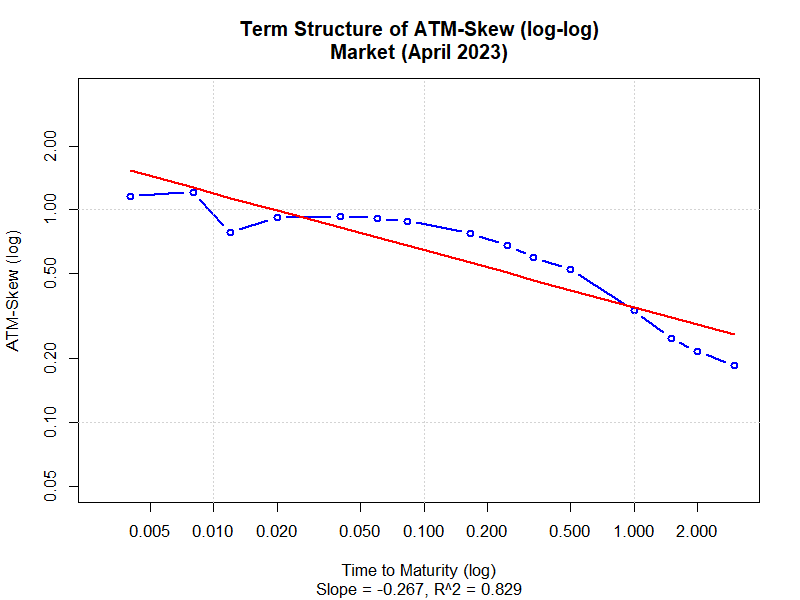
\includegraphics[width=0.45\textwidth]{figures/A.2 Additional Market Surface/market_apr-23_atm_skew_log.png}
    \caption{Empirical implied volatility surface, volatility smiles, and ATM skew (S\&P~500; April 2023).}
    \label{fig:MarketSurfaceApr2023}
\end{figure}


\newpage
\subsection*{A.3\quad Calibration Diagnostics}

\begin{figure}[H]
    \centering
    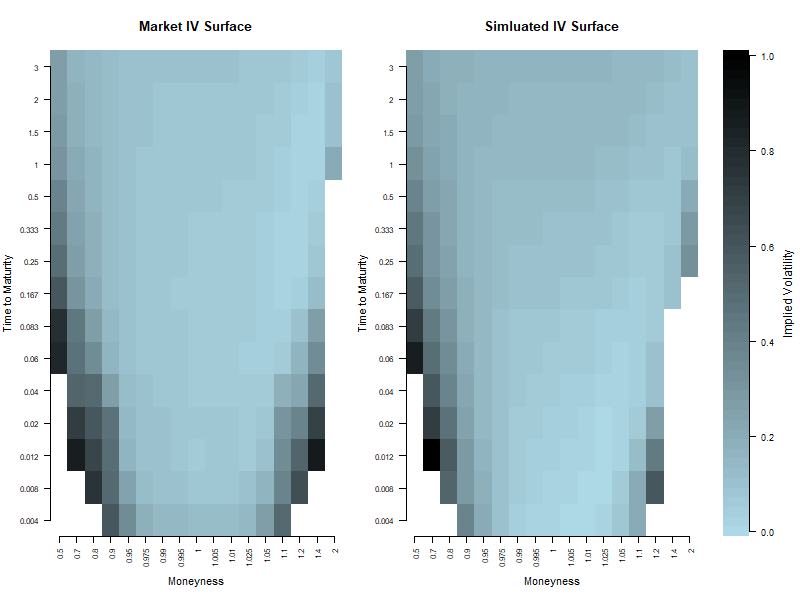
\includegraphics[width=0.75\textwidth]{figures/A.3 Calibration Diagnostics/market_best_fit_heatmap.png}
    \caption{Heatmap comparison of the empirical implied volatility surface (S\&P~500, March 2023) 
    and the calibrated Hypergeometric Volatility Model surface.}
    \label{fig:HeatmapMarketBestFit}
\end{figure}

\begin{figure}[H]
    \centering
    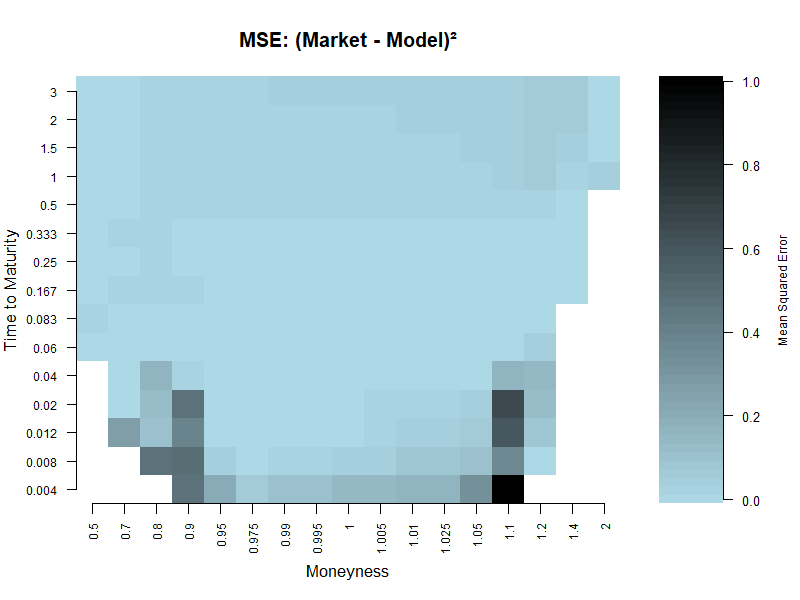
\includegraphics[width=0.75\textwidth]{figures/A.3 Calibration Diagnostics/market_best_fit_mse_heatmap.png}
    \caption{Heatmap of the squared error between the empirical and calibrated implied volatility surfaces. 
    Errors are concentrated in short-maturity and far out-of-the-money regions, 
    highlighting areas where the model struggles to capture market dynamics.}
    \label{fig:HeatmapMarketBestFitMSE}
\end{figure}
